\section{Metamask}\label{section:metamask}
\subsection{Cos'è Metamask}
Metamask è un estensione per browser che ti permette di gestire il tuo wallet digitale di Ethereum e ti permette di inviare e ricevere Ether (Fantom in \projectName{}).
Metamask deve essere installato nel tuo browser per tutto il tempo che userai \projectName{}, senza di esso non potrai usare la nostra piattaforma.
\subsection{Installazione}
Dopo essere entrato in \projectName{}, controlla che Metamask sia installato, puoi farlo guardando se tra le estensioni in alto a destra è presente la sua icona.

    \begin{figure}[htbp]
        \centering
        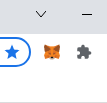
\includegraphics{immagini/metamask_installed.png}
        \caption{Metamask installato correttamente}
    \end{figure}   
 Se Metamask è installato correttamente, puoi procedere con l'utilizzo di \projectName, altrimenti consulta il video nella sezione sottostante (link video installazione metamask) e procedi con l'installazione.

\subsubsection{Configurazione}
Clicca l'icona di Metamask in alto a destra nel tuo browser e imposta il tuo wallet digitale Fantom seguendo le istruzioni.
Puoi creare un account nuovo, oppure importare uno già esistente tramite la frase iniziale di 12 parole che ti è stata precedentemente fornita.

\subsection{Operazioni}
Ogni volta che si effettua una operazione che cambia lo stato del network\glo{} Fantom\glo{}, Metamask andrà ad aprire una finestra pop-up con il costo totale dell'operazione.
Da questa finestra l'utente potrà confermare o rifiutare l'operazione corrente.

%immagine pop up metamask

Ogni cambiamento effettuato sul network Fantom ha un costi, chiamati Gas Fees\glo{}, misurati in WEI\glo{} (10\textsuperscript{-18} FTM).
Questi costi sono fortemente variabili nel tempo e pertanto non prevedibili.

\section{Metamask e ShopChain}

Per utilizzare l'applicazione ShopChain è necessario disporre di un account Metamask impostato sulla testnet Fantom.
Per aggiungere una nuova rete al proprio account Metamask, cliccare su aggiungi rete dal menu in alto a destra del pop-up Metamask;
 si verrà reindirizzati alla pagina apposita per inserire i dati della rete da aggiungere.

 \begin{figure}[H]
    \centering
    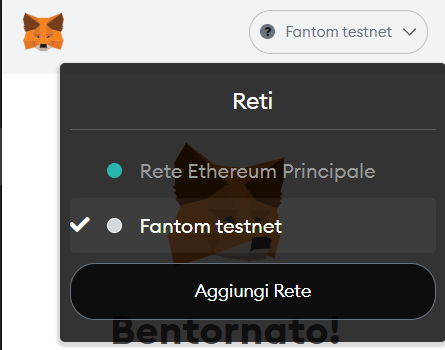
\includegraphics[scale=0.6]{immagini/settmeta1.png}
    \caption{Menu di scelta di rete}
\end{figure} 

I dati da inserire per aggiungere la Fantom Testnet sono i seguenti:

\begin{itemize}
    \item Network Name: Fantom testnet;
    \item New RPC Url: https://rpc.testnet.fantom.network/;
    \item ChainID: 0xfa2
    \item Symbol: FTM
\end{itemize}

\begin{figure}[H]
    \centering
    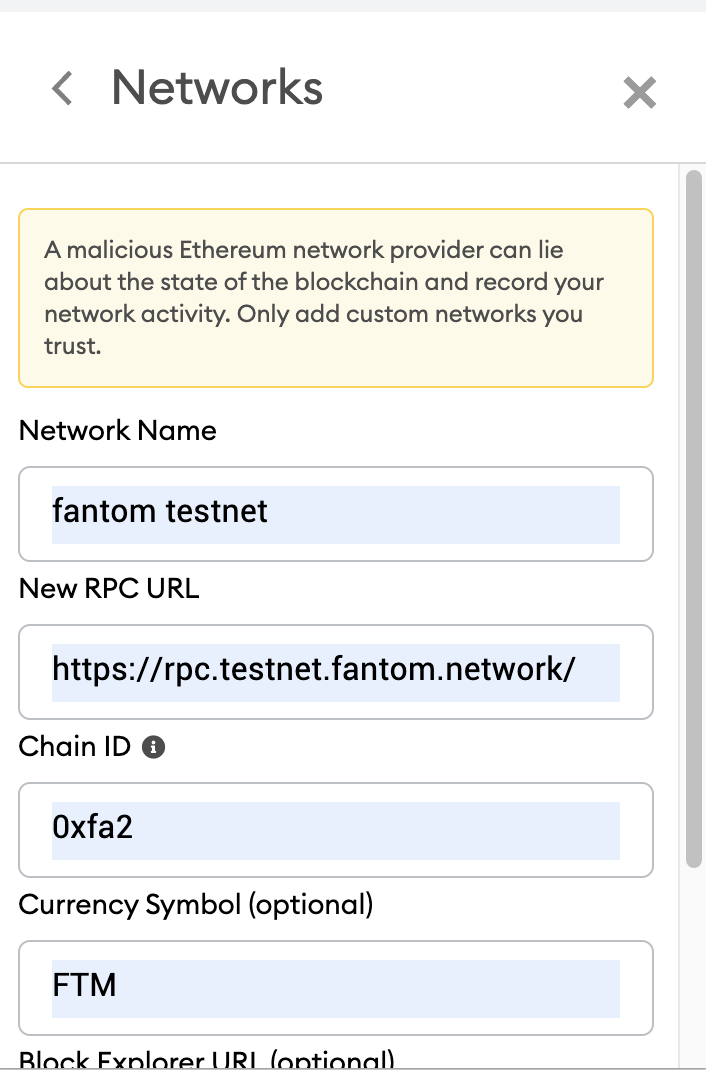
\includegraphics[scale=0.6]{immagini/setmeta2.png}
    \caption{Form per l'aggiunta della rete Fantom Testnet}
\end{figure} 

Appena arrivati alla homepage di ShopChain, è presente una icona in alto a destra che controlla che tutto sia impostato nel modo corretto e, a fianco ad essa, l'indirizzo del wallet del proprio account.
Nel caso la configurazione di metamask non sia stata completata o non eseguita correttamente, l'icona cambierà colore e, posizionando il cursore sulla stessa, verrà mostrato l'errore associato al caso.

%qui figure con gli errori di metamask 